\documentclass[12pt,a4paper]{article}

\usepackage[utf8]{inputenc}
\usepackage[T1]{fontenc}
\usepackage[brazil]{babel}
\usepackage{geometry}
\usepackage{graphicx}
\usepackage{booktabs}
\usepackage{array}
\usepackage{float}
\usepackage{caption}
\usepackage{subcaption}
\usepackage{amsmath}
\usepackage{hyperref}

\geometry{left=2.5cm,right=2.5cm,top=2.5cm,bottom=2.5cm}
\graphicspath{{../}}
\hypersetup{colorlinks=true, linkcolor=blue, urlcolor=blue, citecolor=blue}

\title{Implementação e Avaliação do ClonalG para Agrupamento de Dados}
\author{Computação Natural -- Segundo Trabalho Prático}
\date{Maio de 2026}

\begin{document}
\maketitle

\begin{abstract}
Este relatório apresenta a implementação e a avaliação do algoritmo ClonalG aplicado ao problema de agrupamento de dados. O objetivo foi comparar uma abordagem bioinspirada, baseada em seleção clonal, com o algoritmo clássico k-Médias da biblioteca Scikit-Learn. Foram usados cinco conjuntos de dados, quatro configurações distintas do ClonalG e a métrica Silhouette como critério de qualidade. A análise mostra que o ClonalG conseguiu resultados iguais ou superiores ao k-Médias em alguns cenários, principalmente nos DataSets 2 e 4, mas também mostrou dificuldade no DataSet 3. A discussão destaca o efeito da população, da seleção, da mutação e da memória imunológica sobre os resultados.
\end{abstract}

\tableofcontents
\newpage

\section{Introdução}

Agrupamento de dados é uma tarefa de aprendizado não supervisionado. Nesse tipo de problema, o objetivo é separar exemplos em grupos sem usar rótulos prontos. Um bom agrupamento deve colocar objetos parecidos no mesmo grupo e objetos diferentes em grupos separados.

Neste trabalho foi usado o algoritmo ClonalG, inspirado no funcionamento do sistema imunológico. No sistema imunológico real, células que reconhecem bem um invasor tendem a se multiplicar, sofrer pequenas alterações e gerar células de memória. No algoritmo, a ideia é semelhante: uma população de soluções candidatas é avaliada, as melhores geram clones, os clones sofrem mutações, e as melhores soluções são preservadas para as próximas iterações.

No contexto deste trabalho, cada solução candidata, chamada de anticorpo, representa um conjunto de centroides. Esses centroides definem os grupos. Cada ponto do dataset é associado ao centroide mais próximo, usando distância Euclidiana. A qualidade do agrupamento é medida pelo índice Silhouette.

O ClonalG foi comparado com o k-Médias. O k-Médias é uma técnica clássica de agrupamento baseada em centroides. Ele é simples, rápido e muito usado, mas depende diretamente da escolha do número de grupos \(k\). Já o ClonalG usado neste trabalho permite alterar estruturalmente o número de centroides durante a busca, tentando descobrir um bom valor de \(k\) dentro de um intervalo definido.

\section{Materiais e Métodos}

\subsection{Conjuntos de dados}

Foram utilizados os cinco conjuntos de dados fornecidos para o trabalho. Todos os dados passaram por pré-processamento antes da execução dos algoritmos. A Tabela~\ref{tab:dados} mostra o tamanho final de cada dataset.

\begin{table}[H]
\centering
\caption{Resumo dos conjuntos de dados usados nos experimentos.}
\label{tab:dados}
\begin{tabular}{cccc}
\toprule
DataSet & Amostras & Atributos & Valores ausentes \\
\midrule
1 & 300 & 2 & 0 \\
2 & 1010 & 2 & 0 \\
3 & 300 & 4 & 0 \\
4 & 230 & 2 & 0 \\
5 & 440 & 6 & 0 \\
\bottomrule
\end{tabular}
\end{table}

Antes dos testes, os atributos foram padronizados. Essa etapa é importante porque tanto o ClonalG quanto o k-Médias usam distância Euclidiana. Se uma variável tiver valores muito maiores que outra, ela pode dominar o cálculo da distância e prejudicar o agrupamento.

\subsection{Análise exploratória}

A primeira etapa foi observar a distribuição dos dados. Para datasets com dois atributos, a visualização foi feita diretamente no plano. Para datasets com mais atributos, foi usada uma projeção em duas dimensões apenas para visualizar os pontos. A projeção não foi usada para treinar os algoritmos.

\begin{figure}[H]
\centering
\begin{subfigure}{0.48\textwidth}
\centering
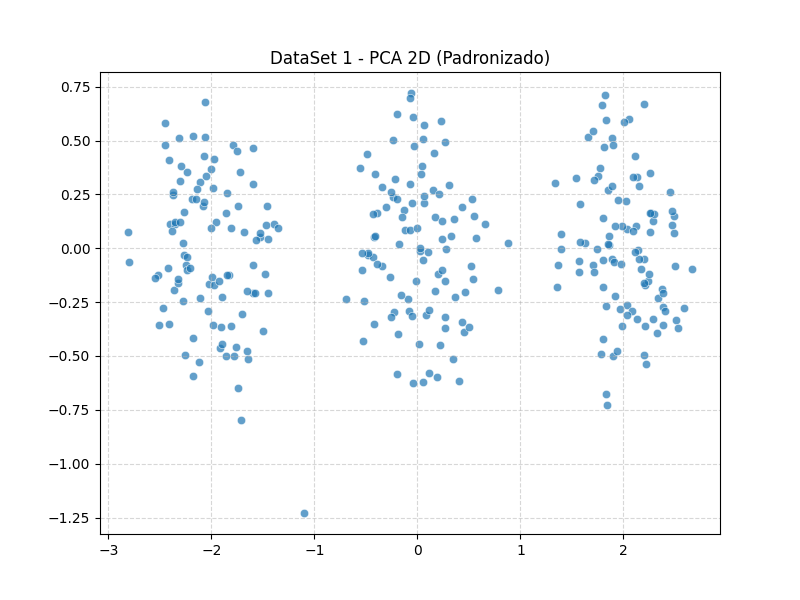
\includegraphics[width=\textwidth]{resultados/etapa1/dataset1_plot.png}
\caption{DataSet 1}
\end{subfigure}
\begin{subfigure}{0.48\textwidth}
\centering
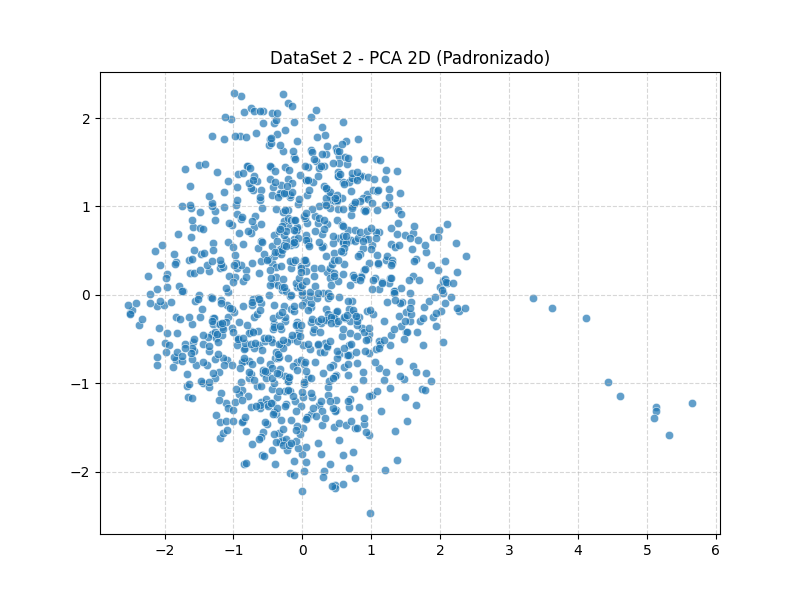
\includegraphics[width=\textwidth]{resultados/etapa1/dataset2_plot.png}
\caption{DataSet 2}
\end{subfigure}

\begin{subfigure}{0.48\textwidth}
\centering
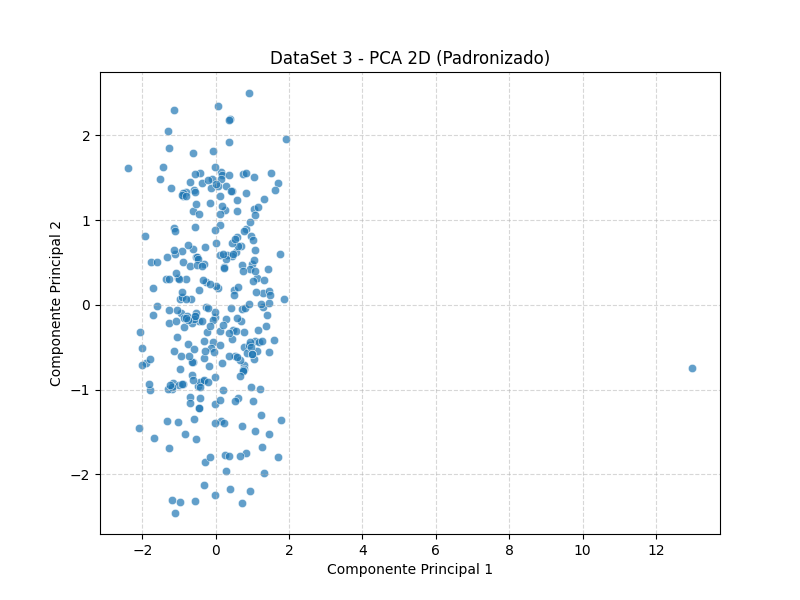
\includegraphics[width=\textwidth]{resultados/etapa1/dataset3_plot.png}
\caption{DataSet 3}
\end{subfigure}
\begin{subfigure}{0.48\textwidth}
\centering
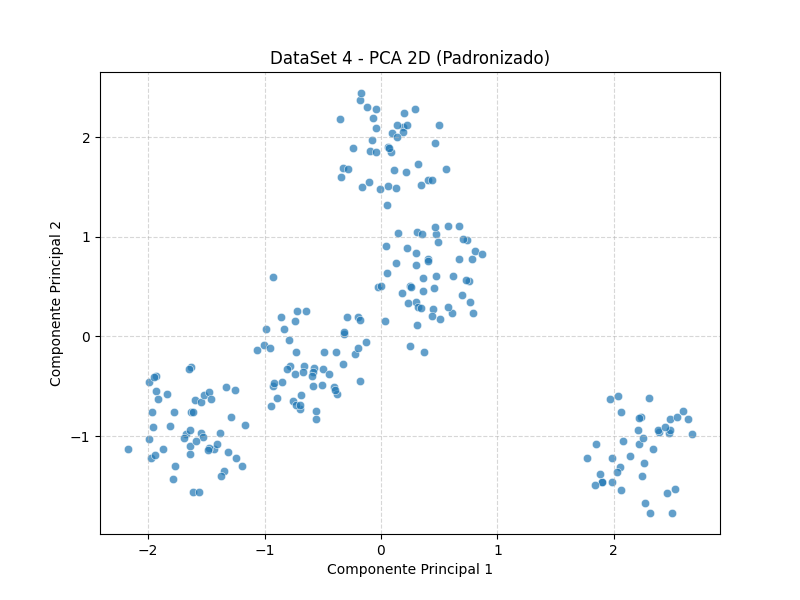
\includegraphics[width=\textwidth]{resultados/etapa1/dataset4_plot.png}
\caption{DataSet 4}
\end{subfigure}

\begin{subfigure}{0.55\textwidth}
\centering
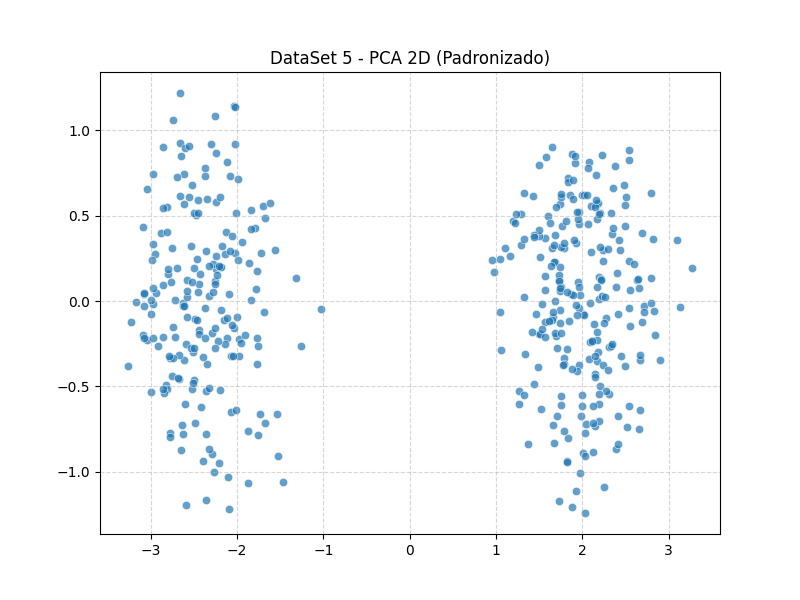
\includegraphics[width=\textwidth]{resultados/etapa1/dataset5_plot.png}
\caption{DataSet 5}
\end{subfigure}
\caption{Visualização inicial dos datasets após pré-processamento.}
\label{fig:exploratoria}
\end{figure}

\subsection{Representação do anticorpo}

No algoritmo implementado, cada anticorpo representa uma possível solução para o agrupamento. Um anticorpo é uma matriz com \(k\) centroides:

\[
A = \{c_1, c_2, \ldots, c_k\}
\]

Cada centroide \(c_j\) possui a mesma quantidade de atributos dos dados. Para classificar um ponto, o algoritmo calcula a distância desse ponto até todos os centroides e escolhe o centroide mais próximo.

\subsection{Índice Silhouette}

O índice Silhouette foi usado como métrica principal de avaliação. Para cada ponto, o Silhouette compara duas ideias:

\begin{itemize}
    \item coesão: o quanto o ponto está próximo dos pontos do próprio grupo;
    \item separação: o quanto o ponto está distante dos pontos do grupo vizinho mais parecido.
\end{itemize}

O valor do Silhouette fica aproximadamente entre \(-1\) e \(1\). Valores mais próximos de \(1\) indicam grupos mais bem definidos. Valores próximos de \(0\) indicam grupos sobrepostos ou pouco separados. Valores negativos indicam que muitos pontos podem estar em grupos inadequados.

\subsection{Processos imunológicos implementados}

O enunciado exige que o ClonalG tenha quatro processos imunológicos principais. Eles foram implementados da seguinte forma:

\begin{itemize}
    \item \textbf{Reconhecimento}: cada anticorpo gera grupos por distância Euclidiana entre os pontos e os centroides. Em seguida, sua afinidade é medida pelo índice Silhouette.
    \item \textbf{Proliferação}: os melhores anticorpos produzem clones. Quanto maior a afinidade normalizada, maior a quantidade de clones.
    \item \textbf{Variação}: os clones sofrem hipermutação. Neste trabalho, a mutação foi estrutural: o clone pode adicionar, remover ou manter centroides, respeitando os limites de \(k\).
    \item \textbf{Seleção e diversidade}: as melhores soluções são preservadas na memória. Parte dos piores indivíduos do repertório é substituída por novos anticorpos aleatórios, evitando que a população fique muito parecida.
\end{itemize}

\subsection{Pseudocódigo}

\begin{verbatim}
Entrada: dados X, candidatos de k, tamanho da população N,
         rho, beta, taxa de seleção, taxa de substituição,
         número de iterações

Para cada valor inicial de k:
    Criar população inicial de anticorpos
    Calcular afinidade inicial por Silhouette
    Separar memória e repertório

    Para cada iteração:
        Selecionar os melhores anticorpos da memória
        Para cada anticorpo selecionado:
            Gerar clones proporcionalmente a afinidade
            Aplicar hipermutação estrutural nos clones
        Calcular afinidade dos clones
        Combinar memória, repertório e clones
        Manter os melhores na memória
        Substituir parte dos piores indivíduos por novos anticorpos

    Guardar o melhor resultado obtido

Comparar o melhor ClonalG com o k-Médias usando o mesmo k final.
\end{verbatim}

\subsection{Configurações testadas}

Foram avaliadas quatro configurações distintas do ClonalG, armazenadas nas pastas \texttt{resultados/resultados}, \texttt{resultados/resultados2}, \texttt{resultados/resultados3} e \texttt{resultados/resultados4}. Todas usaram os candidatos de \(k = \{2,3,4,5,6\}\), 3 repetições por dataset e 50 iterações por execução.

\begin{table}[H]
\centering
\caption{Configurações comparadas nos experimentos.}
\label{tab:configs}
\resizebox{\textwidth}{!}{%
\begin{tabular}{cccccccc}
\toprule
Config. & Pasta & Anticorpos \(N\) & \(\rho\) & \(\beta\) & Substituição & Seleção & Interpretação \\
\midrule
C1 & resultados & 15 & 2.0 & 15.0 & 0.10 & 0.85 & Menor diversidade e seleção alta \\
C2 & resultados2 & 15 & 2.0 & 5.0 & 0.30 & 0.50 & Menos clones e mais substituição \\
C3 & resultados3 & 30 & 2.0 & 15.0 & 0.30 & 0.30 & População maior e seleção mais restrita \\
C4 & resultados4 & 60 & 3.5 & 30.0 & 0.40 & 0.60 & Busca mais intensa e população maior \\
\bottomrule
\end{tabular}%
}
\end{table}

O parâmetro \(N\) controla o tamanho da população. O parâmetro \(\rho\) controla a intensidade da hipermutação inversamente proporcional à afinidade. O parâmetro \(\beta\) controla a quantidade de clones. A taxa de substituição aumenta a diversidade, trocando indivíduos fracos por novos candidatos. A taxa de seleção controla quantos indivíduos bons participam da clonagem.

\section{Resultados e Discussão}

\subsection{Visão geral das quatro configurações}

A Figura~\ref{fig:quatro-configs} compara o Silhouette médio das quatro configurações em cada dataset. A linha preta mostra o resultado do k-Médias usando o mesmo \(k\) encontrado pelo ClonalG.

\begin{figure}[H]
\centering
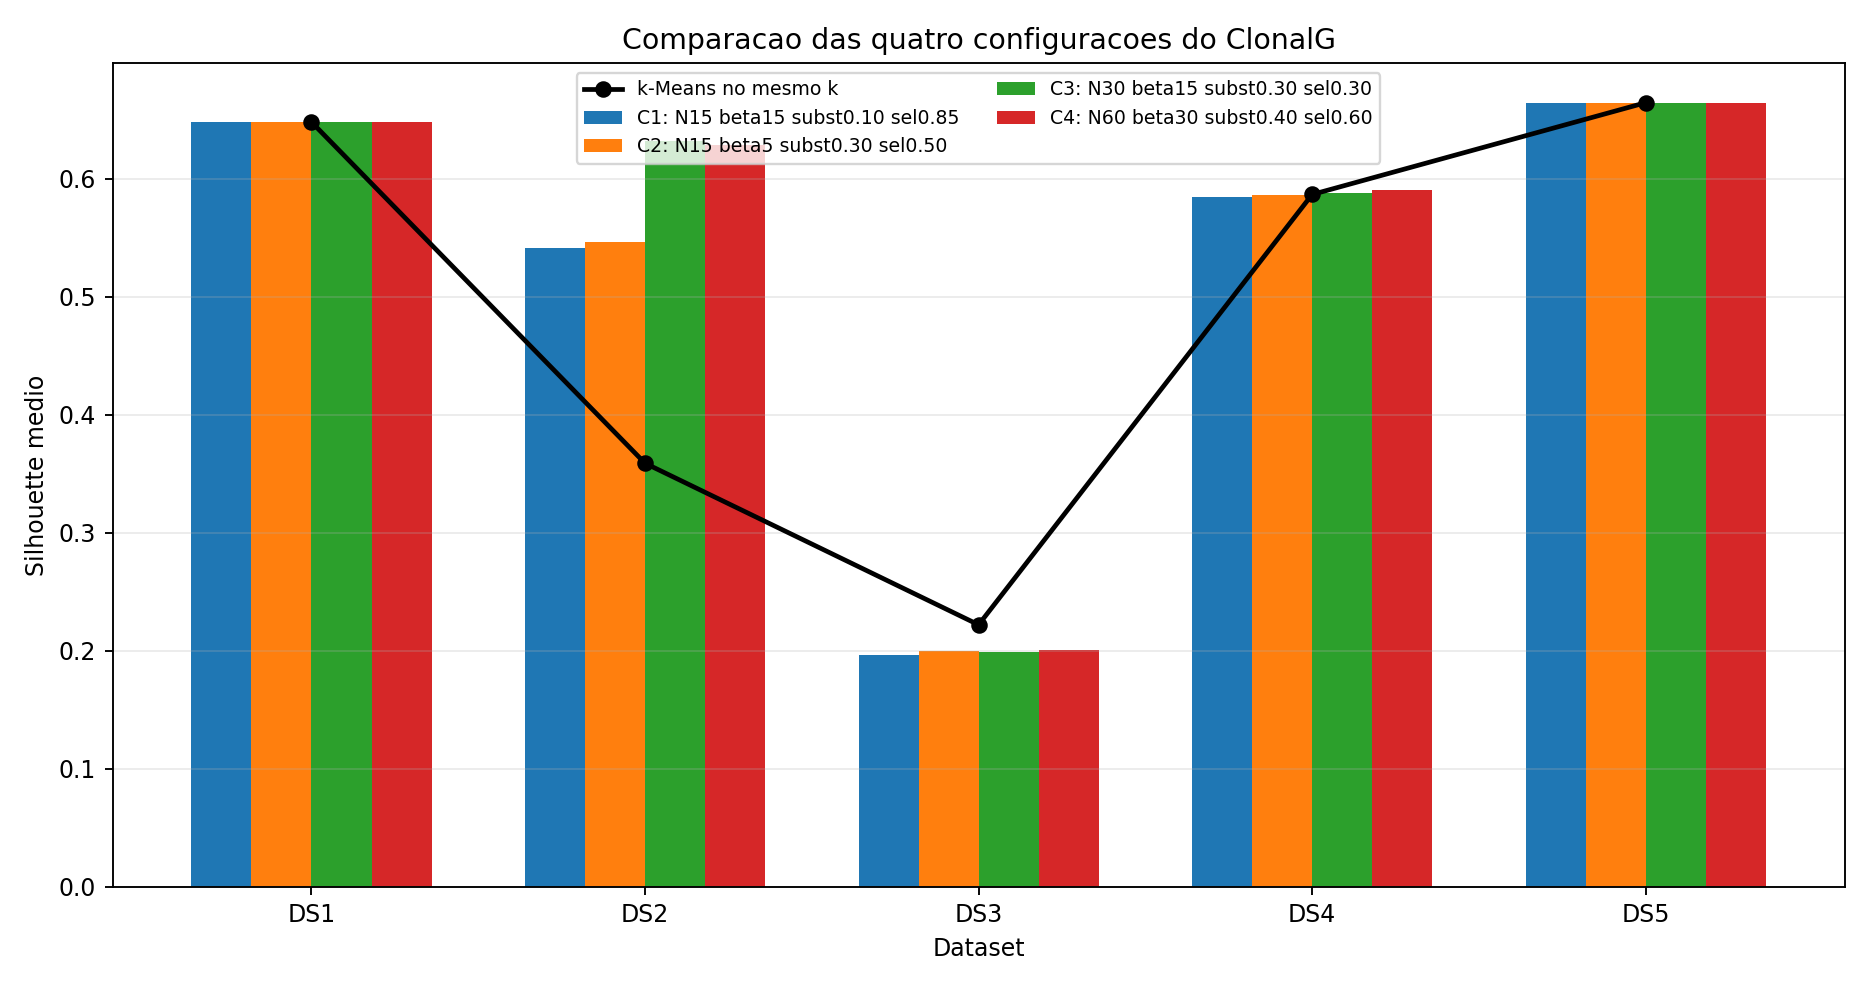
\includegraphics[width=\textwidth]{resultados/comparativo_quatro_configuracoes.png}
\caption{Comparação geral das quatro configurações do ClonalG com o k-Médias.}
\label{fig:quatro-configs}
\end{figure}

O resultado geral mostra três comportamentos diferentes. Nos DataSets 1 e 5, todas as configurações chegaram ao mesmo resultado que o k-Médias. No DataSet 2, o ClonalG superou o k-Médias com boa margem, principalmente nas configurações C3 e C4. No DataSet 3, o k-Médias foi melhor que todas as configurações do ClonalG. No DataSet 4, o ClonalG ficou muito próximo do k-Médias nas configurações C1 e C2, e superou levemente o k-Médias nas configurações C3 e C4.

\subsection{Tabela comparativa por dataset}

A Tabela~\ref{tab:comparacao-detalhada} apresenta os principais resultados numéricos. O campo \(\Delta\) é calculado como:

\[
\Delta = Silhouette_{ClonalG} - Silhouette_{k\text{-}Médias}
\]

Logo, valores positivos indicam vantagem do ClonalG, valores negativos indicam vantagem do k-Médias, e zero indica empate.

\begin{table}[H]
\centering
\caption{Comparação detalhada das configurações por dataset.}
\label{tab:comparacao-detalhada}
\resizebox{\textwidth}{!}{%
\begin{tabular}{cccccccc}
\toprule
DataSet & Config. & \(k\) final & \(k\) inicial melhor & ClonalG médio & Melhor ClonalG & k-Médias & \(\Delta\) \\
\midrule
1 & C1 & 3 & 2 & 0.6480 & 0.6480 & 0.6480 & 0.0000 \\
1 & C2 & 3 & 3 & 0.6480 & 0.6480 & 0.6480 & 0.0000 \\
1 & C3 & 3 & 2 & 0.6480 & 0.6480 & 0.6480 & 0.0000 \\
1 & C4 & 3 & 2 & 0.6480 & 0.6480 & 0.6480 & 0.0000 \\
\midrule
2 & C1 & 2 & 4 & 0.5417 & 0.6158 & 0.3589 & 0.1827 \\
2 & C2 & 2 & 5 & 0.5462 & 0.6158 & 0.3589 & 0.1872 \\
2 & C3 & 2 & 5 & 0.6318 & 0.6637 & 0.3589 & 0.2729 \\
2 & C4 & 2 & 6 & 0.6285 & 0.6539 & 0.3589 & 0.2696 \\
\midrule
3 & C1 & 6 & 4 & 0.1969 & 0.2041 & 0.2221 & -0.0252 \\
3 & C2 & 5 & 3 & 0.1995 & 0.2078 & 0.2220 & -0.0225 \\
3 & C3 & 5 & 3 & 0.1992 & 0.2048 & 0.2220 & -0.0229 \\
3 & C4 & 6 & 2 & 0.2006 & 0.2066 & 0.2221 & -0.0215 \\
\midrule
4 & C1 & 4 & 4 & 0.5847 & 0.5898 & 0.5866 & -0.0018 \\
4 & C2 & 4 & 3 & 0.5865 & 0.5904 & 0.5866 & -0.0001 \\
4 & C3 & 4 & 6 & 0.5877 & 0.5894 & 0.5866 & 0.0011 \\
4 & C4 & 4 & 4 & 0.5902 & 0.5905 & 0.5866 & 0.0036 \\
\midrule
5 & C1 & 2 & 2 & 0.6644 & 0.6644 & 0.6644 & 0.0000 \\
5 & C2 & 2 & 2 & 0.6644 & 0.6644 & 0.6644 & 0.0000 \\
5 & C3 & 2 & 2 & 0.6644 & 0.6644 & 0.6644 & 0.0000 \\
5 & C4 & 2 & 2 & 0.6644 & 0.6644 & 0.6644 & 0.0000 \\
\bottomrule
\end{tabular}%
}
\end{table}

\subsection{Melhores parâmetros por dataset}

Um dos pontos pedidos no enunciado é apresentar os melhores parâmetros finais para cada dataset. A Tabela~\ref{tab:melhores-parametros} mostra a configuração com maior Silhouette médio do ClonalG em cada caso.

\begin{table}[H]
\centering
\caption{Melhores parâmetros encontrados para cada dataset.}
\label{tab:melhores-parametros}
\resizebox{\textwidth}{!}{%
\begin{tabular}{cccccccccc}
\toprule
DataSet & Config. & \(k\) final & \(N\) & \(\rho\) & \(\beta\) & Subst. & Sel. & ClonalG & \(\Delta\) \\
\midrule
1 & C1 & 3 & 15 & 2.0 & 15.0 & 0.10 & 0.85 & 0.6480 & 0.0000 \\
2 & C3 & 2 & 30 & 2.0 & 15.0 & 0.30 & 0.30 & 0.6318 & 0.2729 \\
3 & C4 & 6 & 60 & 3.5 & 30.0 & 0.40 & 0.60 & 0.2006 & -0.0215 \\
4 & C4 & 4 & 60 & 3.5 & 30.0 & 0.40 & 0.60 & 0.5902 & 0.0036 \\
5 & C1 & 2 & 15 & 2.0 & 15.0 & 0.10 & 0.85 & 0.6644 & 0.0000 \\
\bottomrule
\end{tabular}%
}
\end{table}

Esses resultados mostram que não houve uma configuração única claramente melhor para todos os datasets. Isso é esperado em algoritmos bioinspirados, porque a melhor combinação entre exploração e explotação depende da forma dos dados. Mesmo assim, as configurações C3 e C4 tiveram as melhores médias gerais, principalmente por melhorarem os DataSets 2 e 4.

\subsection{Discussão por dataset}

\subsubsection*{DataSet 1}

No DataSet 1, todas as configurações encontraram \(k=3\) e obtiveram Silhouette 0.6480, exatamente igual ao k-Médias. Esse comportamento indica que a estrutura dos grupos é bem definida e fácil de encontrar. Aumentar população, clonagem ou substituição não trouxe ganho, pois a configuração mais simples já chegou ao mesmo agrupamento de qualidade.

Nesse caso, o k-Médias é competitivo por ser direto e rápido. O ClonalG também funcionou corretamente, mas seu custo computacional é maior. Portanto, para um dataset com grupos bem separados e estrutura simples, o ClonalG não trouxe vantagem prática sobre o k-Médias.

\subsubsection*{DataSet 2}

O DataSet 2 foi o caso em que o ClonalG mais superou o k-Médias. O k-Médias obteve Silhouette 0.3589 com o mesmo \(k\), enquanto o ClonalG chegou à média 0.6318 na configuração C3. O ganho foi de 0.2729, que é uma diferença relevante.

A diferença entre as configurações mostra o efeito dos parâmetros. C1 e C2 usaram apenas 15 anticorpos e ficaram em torno de 0.54. Quando a população aumentou para 30 anticorpos em C3, a média subiu para 0.6318. C4, com 60 anticorpos, também foi forte, mas ficou levemente abaixo de C3. Isso sugere que aumentar a população ajudou a explorar melhores soluções, mas aumentar demais a intensidade da busca não garantiu melhora adicional.

Outro ponto importante é que o melhor \(k\) final foi 2, mesmo quando o melhor \(k\) inicial variou entre 4, 5 e 6. Isso mostra que a mutação estrutural conseguiu ajustar o número de centroides durante a busca. Portanto, neste dataset, o ClonalG lidou bem com o desafio de descobrir o número de clusters dentro do intervalo permitido.

\subsubsection*{DataSet 3}

O DataSet 3 foi o caso mais difícil para o ClonalG. Todas as configurações ficaram abaixo do k-Médias. A melhor configuração foi C4, com Silhouette médio 0.2006, enquanto o k-Médias ficou em 0.2221. A diferença não é enorme, mas foi consistente contra o ClonalG.

Esse resultado indica que, para esse dataset, a busca populacional e a mutação estrutural não encontraram uma solução melhor que o particionamento direto do k-Médias. Como o DataSet 3 tem quatro atributos, a estrutura pode ser menos evidente na representação por centroides mutados apenas por adição ou remoção. Também é possível que o intervalo de \(k\) ou a forma de mutação usada não tenha sido suficiente para explorar melhor esse espaço.

Mesmo com população maior e mutação mais forte em C4, o ganho foi pequeno. Isso mostra que aumentar parâmetros não resolve todos os casos. Em alguns problemas, a estratégia de mutação ou a função de afinidade podem precisar de ajustes mais específicos.

\subsubsection*{DataSet 4}

No DataSet 4, o ClonalG e o k-Médias ficaram muito próximos. C1 ficou um pouco abaixo do k-Médias, C2 praticamente empatou, e C3 e C4 superaram levemente o k-Médias. A melhor média foi C4, com 0.5902 contra 0.5866 do k-Médias.

Esse caso mostra uma melhora pequena, mas coerente com o aumento da capacidade de exploração. A configuração C4 tinha maior população, maior fator de clonagem, maior taxa de substituição e maior \(\rho\). Esses parâmetros aumentaram a diversidade e a pressão de busca, permitindo encontrar uma solução um pouco melhor.

Mesmo assim, a diferença é pequena. Portanto, a conclusão correta não é que o ClonalG dominou o k-Médias nesse dataset, mas que ele conseguiu desempenho competitivo e levemente superior na melhor configuração.

\subsubsection*{DataSet 5}

No DataSet 5, todas as configurações encontraram \(k=2\) e obtiveram Silhouette 0.6644, igual ao k-Médias. Isso indica estabilidade. A qualidade não dependeu muito dos parâmetros testados.

Esse comportamento é parecido com o DataSet 1: quando a estrutura dos grupos é clara para uma abordagem baseada em centroides, tanto o ClonalG quanto o k-Médias chegam a resultados equivalentes. Nesse caso, a memória imunológica preservou a melhor solução, mas não houve necessidade de uma exploração mais agressiva.

\subsection{Efeito dos parâmetros}

O tamanho da população afetou principalmente os DataSets 2 e 4. Em C1 e C2, com \(N=15\), o ClonalG teve menor capacidade de explorar soluções diferentes. Em C3, com \(N=30\), houve grande melhora no DataSet 2. Em C4, com \(N=60\), houve melhora no DataSet 4 e pequena melhora no DataSet 3, mas não superou C3 no DataSet 2.

A taxa de seleção também teve efeito importante. Uma seleção muito alta, como em C1, usa muitos bons indivíduos na clonagem, mas pode reduzir a variedade das soluções se a memória ficar dominada por candidatos parecidos. Uma seleção menor, como em C3, torna a clonagem mais concentrada em poucos candidatos fortes e pode ajudar quando combinada com substituição maior.

O fator de mutação \(\rho\) e o fator de clonagem \(\beta\) influenciam o equilíbrio entre busca local e busca global. C4 usou \(\rho=3.5\) e \(\beta=30\), gerando uma busca mais intensa. Isso ajudou no DataSet 4 e produziu a melhor configuração para o DataSet 3, mas não resolveu totalmente o problema desse dataset. Assim, a configuração mais agressiva não foi universalmente melhor.

A taxa de substituição ajudou a manter diversidade. C1 tinha substituição 0.10, enquanto C3 e C4 usaram 0.30 e 0.40. Nos datasets em que o ClonalG precisou escapar de soluções piores, como o DataSet 2, essa diversidade foi importante.

\subsection{Descoberta do número de clusters}

O enunciado pergunta se o ClonalG consegue lidar organicamente com o número de clusters. Neste trabalho, ele não escolhe \(k\) de forma totalmente livre, pois recebe um intervalo de candidatos entre 2 e 6. No entanto, dentro desse intervalo, a mutação estrutural permite adicionar ou remover centroides.

Os resultados mostram que essa estratégia funcionou em vários casos. No DataSet 2, por exemplo, diferentes \(k\) iniciais levaram ao \(k=2\) final, que foi o melhor resultado. No DataSet 4, o algoritmo convergiu para \(k=4\). Nos DataSets 1 e 5, as configurações foram estáveis em \(k=3\) e \(k=2\), respectivamente.

Portanto, a resposta mais adequada é: o ClonalG implementado consegue ajustar \(k\) organicamente dentro de limites definidos pelo usuário. Ele ainda precisa de intervenção para definir o intervalo permitido, mas não depende de um único \(k\) fixo desde o início.

\subsection{Memória imunológica}

A memória imunológica é a parte do algoritmo que preserva os melhores anticorpos ao longo das gerações. Sem memória, uma boa solução encontrada em uma iteração poderia ser perdida nas próximas mutações. Com memória, o algoritmo mantém as melhores soluções e usa essas soluções como base para novas clonagens.

Nos DataSets 1 e 5, a memória ajudou a manter resultados estáveis. Como os agrupamentos eram bem definidos, uma vez encontrada a boa solução, ela foi preservada. No DataSet 2, a memória foi importante para acumular boas soluções enquanto a substituição mantinha diversidade na população. Isso ajudou o ClonalG a superar o k-Médias.

Por outro lado, a memória também pode causar convergência prematura. Se os primeiros bons anticorpos não forem realmente bons em termos globais, a população pode ficar concentrada ao redor de soluções medianas. Por isso a taxa de substituição é importante: ela insere novos anticorpos e reduz o risco de a memória dominar completamente a busca.

\subsection{Comparação técnica com k-Médias}

O k-Médias foi melhor no DataSet 3 e empatou nos DataSets 1 e 5. Ele é mais simples e tende a ser mais rápido, pois não trabalha com população, clonagem e várias repetições de avaliação. Em problemas com grupos bem representados por centroides, ele é uma referência muito forte.

O ClonalG foi melhor no DataSet 2 e levemente melhor no DataSet 4. Sua vantagem aparece quando a busca populacional consegue explorar alternativas que o k-Médias não encontra tão facilmente. O custo é maior, pois cada anticorpo e cada clone precisam ser avaliados por Silhouette. Portanto, o ClonalG oferece maior flexibilidade, mas exige mais cuidado com parâmetros e tempo de execução.

\section{Conclusão}

O trabalho implementou e avaliou o ClonalG para agrupamento de dados, incluindo reconhecimento por distância Euclidiana, proliferação proporcional à afinidade, hipermutação inversamente proporcional à afinidade, seleção, substituição de indivíduos fracos e memória imunológica.

Os experimentos com quatro configurações mostraram que o ClonalG é competitivo com o k-Médias. Ele empatou nos DataSets 1 e 5, superou claramente o k-Médias no DataSet 2, superou levemente no DataSet 4 e foi superado no DataSet 3. A melhor configuração geral ficou entre C3 e C4, mas a melhor escolha dependeu do dataset.

A análise dos parâmetros mostrou que população maior e maior substituição podem melhorar a exploração, mas também aumentam custo computacional. O algoritmo conseguiu ajustar o número de clusters dentro do intervalo permitido, o que responde ao desafio do enunciado: ele não descobre \(k\) de forma totalmente independente, mas consegue modificar \(k\) durante a busca.

Como melhoria futura, seria interessante testar outras formas de mutação, executar mais repetições, incluir tempo médio de execução e comparar também com outras métricas de validação interna além do Silhouette.

\end{document}
